\documentclass[12pt, twoside]{article}
\documentclass[12pt, twoside]{article}
\usepackage[letterpaper, margin=1in, headsep=0.2in]{geometry}
\setlength{\headheight}{0.6in}
%\usepackage[english]{babel}
\usepackage[utf8]{inputenc}
\usepackage{microtype}
\usepackage{amsmath}
\usepackage{amssymb}
%\usepackage{amsfonts}
\usepackage{siunitx} %units in math. eg 20\milli\meter
\usepackage{yhmath} % for arcs, overparenth command
\usepackage{tikz} %graphics
\usetikzlibrary{quotes, angles}
\usepackage{graphicx} %consider setting \graphicspath{{images/}}
\usepackage{parskip} %no paragraph indent
\usepackage{enumitem}
\usepackage{multicol}
\usepackage{venndiagram}

\usepackage{fancyhdr}
\pagestyle{fancy}
\fancyhf{}
\renewcommand{\headrulewidth}{0pt} % disable the underline of the header
\raggedbottom
\hfuzz=2mm %suppresses overfull box warnings

\usepackage{hyperref}
\usepackage{float}

\title{Algebra 2}
\author{Chris Huson}
\date{June 2024}

\fancyhead[LE]{\thepage}
\fancyhead[RO]{\thepage \\ Name: \hspace{1.5cm} \,\\}
\fancyhead[LO]{BECA/Huson/Algebra 2: Regents Preparation \\* 11 June 2024}

\begin{document}
\subsubsection*{Prep \#27 Inverse functions}
\begin{enumerate}
\item The line $y=x$ is shown on the graph below.
    \begin{enumerate}
        \item Graph and label the function $f(x)=2^x$.
        \item Graph and label its inverse $f^{-1}(x)=\log_2{x}$.
        \item Mark and label the following points on the appropriate curves:\\
         $(0,1)$, $(2,4)$, $(3,8)$ and $(1,0)$, $(4,2)$, $(8,3)$
    \end{enumerate}
    \begin{center}
        \begin{tikzpicture}[scale=1.2]
        \draw[gray,thin] (-4,-4) grid[xstep=1,ystep=1] (8,8);
        \draw [thick,->] (-4,0)--(8.3,0) node [above] {$x$};
        \draw [thick,->] (0,-4)--(0,8.5) node [above] {$y$};
        \foreach \x in {-4,-2,2,4,...,8}
            \draw (\x,5pt) -- (\x,-5pt) node[below] {$\x$};
        \foreach \y in {-4,-2,2,4,...,8}
            \draw (2pt,\y cm)--(-2pt,\y cm) node[left]{$\y$};
        \draw [thick,dashed,<->, domain=-3.5:7.5,smooth,samples=100] plot (\x,{\x});
        %\draw [thick,->, domain=-3:3.1,smooth,samples=100] plot (\x,{2^\x});
        %\draw [thick,->, domain=0.125:8.3,smooth,samples=100] plot (\x,{log2(\x)});
            \end{tikzpicture}
        \end{center}

\newpage
\item The line $y=x$ is shown on the graph below.
    \begin{enumerate}
        \item Graph and label the function $f(x)=x^2$.
        \item Graph and label its inverse $f^{-1}(x)=\sqrt{x}$.
        \item Mark and label the following points on the appropriate curves:\\
        $(2,4)$ and $(4,2)$, $(3,9)$ and $(9,3)$
    \end{enumerate}
    \begin{center}
        \begin{tikzpicture}[scale=1.0]
            \draw[gray,thin] (-4,-4) grid[xstep=1,ystep=1] (9,9);
            \draw [thick,->] (-4,0)--(9.3,0) node [above] {$x$};
            \draw [thick,->] (0,-4)--(0,9.5) node [above] {$y$};
            \foreach \x in {-4,-2,2,4,...,8}
                \draw (\x,5pt) -- (\x,-5pt) node[below] {$\x$};
            \foreach \y in {-4,-2,2,4,...,8}
                \draw (2pt,\y cm)--(-2pt,\y cm) node[left]{$\y$};
            \draw [thick,dashed,<->, domain=-3.5:8.5,smooth,samples=100] plot (\x,{\x});
            %\draw [thick,->, domain=-1:3.0,smooth,samples=100] plot (\x,{\x^2});
            %\draw [thick,->, domain=0:8.2,smooth,samples=100] plot (\x,{sqrt(\x)});
            \end{tikzpicture}
        \end{center}

\newpage

\item Biologists create a culture with 2000 microbes initially. The number of microbes will double every 12 hours. Write an equation for the
number of microbes, $M$, after $t$ hours.
\vspace{2cm}

\item Larry made a \$5000 investment earning an annual rate of 4.80\% compounded monthly.
    \begin{enumerate}
    \item Determine the value of the investment after 5 years using the formula 
        $$\displaystyle V(t)=5000 \times (1+\frac{0.048}{12})^{12t}$$. \vspace{4cm}
    \item Find the time needed for the investment value to reach \$8000, to the \emph{nearest month}. \vspace{4cm}
    \item Susie made a similar investment of \$5000, earning 5.2\% per annum compounded quarterly. Find its value after 5 years, rounded to the \emph{nearest dollar}.
    \end{enumerate}

\newpage
\item Solve the system of equations algebraically. \\[0.25cm] 
    (hint: substitute the value of $y$ from the second equation into the first equation)
    $$\left(x-2\right)^{2}+\left(y-1\right)^{2}=5$$
    $$y=x-2$$

    
\end{enumerate}
\end{document}